\section{李超线段树}
	\href{https://oi-wiki.org/ds/li-chao-tree/}{Luogu-P4097 Segment} \par 
	要求在平面直角坐标系下维护两个操作:\par
	\begin{enumerate}
		\item 在平面上加入一条线段。记第 $i$ 条被插入的线段的标号为 $i$。
		\item 给定一个数 $k$,询问与直线 $x = k$ 相交的线段中,交点纵坐标最大的线段的编号。特别地,若不存在线段与给定直线相交,输出 $0$。
	\end{enumerate}
\subsection{概述}
我们设法维护每个区间中,可能成为最优解的线段。

称一条线段在 $x=x_0$ 处最优,当且仅当该线段在 $x_0$ 处取值最大。

称一条线段能成为区间 $[l,r]$ 中的 最优线段,当且仅当:
\begin{enumerate}
	\item 该线段的定义域完整覆盖了区间 $[l, r]$;
	\item 该线段在区间中点处最优。
\end{enumerate}
现在我们需要插入一条线段,在这条线段完整覆盖的区间中,某些区间的最优线段可能发生改变。
考虑某个被新线段完整覆盖的区间,若该区间无最优线段,则该线段可以直接成为最优线段。

否则,设该区间的中点为 $mid$,我们拿新线段在中点处的值与原最优线段在中点处的值作比较。

首先,如果新线段斜率大于原线段,

如果新线段在 $mid$ 处更优,则新线段在右半区间 \textbf{一定}  最优,旧线段在左半区间 \textbf{可能}  最优;
反之,旧线段在左半区间 \textbf{一定}  最优,新线段在右半区间 \textbf{可能}  最优。
结合图片理解一下(红色线段代表原来的最优线段,黑色线段代表新插入的线段,绿色直线则代表 $x=mid$ 这条直线):
\begin{figure}[htbp]
	\centering
	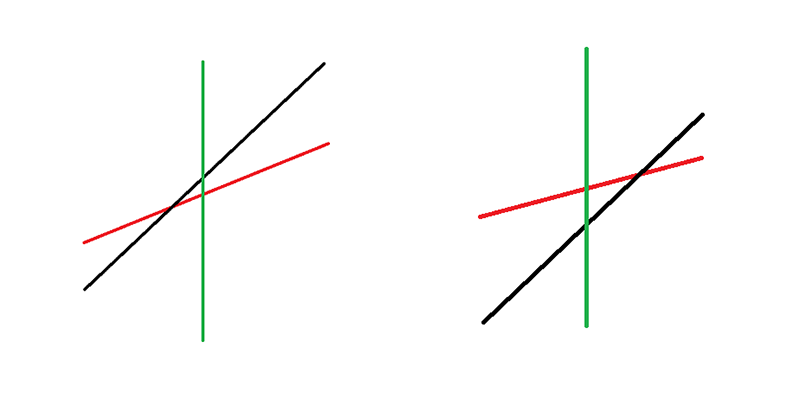
\includegraphics[scale = 0.5]{./image/li-chao-tree1.png}
\end{figure}

	接下来考虑新线段斜率小于原线段的情况,

	如果新线段在 $mid$ 处更优,则新线段在左半区间 \textbf{一定} 最优,旧线段在右半区间 \textbf{可能} 最优;
	反之,旧线段在右半区间 \textbf{一定} 最优,新线段在左半区间 \textbf{可能} 最优。
	再来两张图:
	\begin{figure}[htbp]
		\centering
		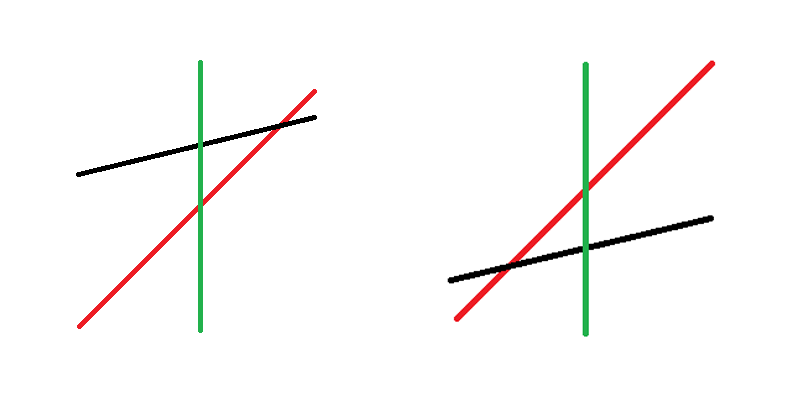
\includegraphics[scale = 0.5]{./image/li-chao-tree2.png}
	\end{figure}
	
	最后考虑新线段和旧线段斜率相同的情况,此时只需比较截距即可,截距大的一定在整个区间内更优。
	
	确定完当前区间的最优线段后,我们需要递归进入子区间,更新最优线段可能改变的区间。
	
	这样的过程与一般线段树的递归过程类似,因此我们可以使用线段树来维护。
	
	现在考虑如何查询一个区间的最优线段。
	
	查询过程利用了标记永久化的思想,简单地说,我们将所有包含 $x_0$ 区间(易知这样的区间只有 $O(\log n)$ 个)的最优线段拿出来,在这些线段中比较,从而得出最优线段。
	
	根据上面的描述,查询过程的时间复杂度显然为 $O(\log n)$,而插入过程中,我们需要将原线段分割到 $O(\log n)$ 个区间中,对于每个区间,我们又需要花费 $O(\log n)$ 的时间更新该区间以及其子区间的最优线段,从而插入过程的时间复杂度为 $O(\log^2 n)$。
	
	